\documentclass[11pt]{article}    % тип дока
\usepackage[utf8]{inputenc}   % используемые языки
\usepackage[T2A]{fontenc}   % используемые языки
\usepackage[english, russian]{babel}   % используемые языки
\usepackage[14pt]{extsizes}   % размер шрифта 14pt
\usepackage[a4paper, left=3cm, right=1cm, top=2cm , bottom=2cm]{geometry}
\usepackage{indentfirst}   % красная строка даже в первом абзаце
\usepackage{graphicx}
\usepackage{xcolor} % пакет для работы с цветами
\usepackage{amssymb}
\usepackage{amsmath}
\usepackage{amsfonts}
\usepackage{hyperref}
\linespread{1.5}   % межстрочный интервал 1.5


\begin{document}

\begin{titlepage}
    
\includegraphics[scale = 0.43]{alf4.JPG}
    \\

НАПРАВЛЕНИЕ 03.03.01 Прикладные математика и физика
\par ПРОФИЛЬ Теоретическая Физика\\

\begin{center}
\begin{bf}
     ЗАДАНИЕ\\
     о прохождении производственной практики (НИР)
\end{bf}



студента Кононова Александра Михайловича \\

Курс 3 Группа 301.3
\end{center}

Форма обучения: очная \\
Сроки прохождения практики с 01.07.2025 по 14.08.2025 \\
Форма представления на кафедру выполненного задания:
отчет в письменной форме\\
Дата выдачи задания: 01.07.2025\\
Задание для прохождения производственной практики (НИР):
Управление многофотонными состояниями, испускаемыми двухуровневой системой\\
С заданием ознакомлен \\

Оценка \\
Руководитель практики Крайнов И.В.\\
(Ф.И.О. полностью, должность, звание, подпись).

\end{titlepage}

\begin{titlepage}


\includegraphics[scale = 0.43]{alf4.JPG}

\

\

\

\

\

\

\begin{center}
    {\bf ОТЧЕТ по производственной практике (НИР)}

    {\bf Весенний семестр 2024/2025 учебного года}

    {\bf Тема: Управление многофотонными состояниями, испускаемыми двухуровневой системой.}

\end{center}

    {\bf Студент: Кононов Александр Михайлович}

    {\bf Руководитель практики: Крайнов Игорь Вадимович}

    {\bf Должность, звание:}

    {\bf Оценка:}

\end{titlepage}

\tableofcontents
\newpage

\section{Введение}
\subsection{Актуальность}

Источники запутанных многофотонных состояний являются ключевыми элементами
квантовых фотонных технологий: линейно-оптических квантовых вычислений,
квантовой криптографии и квантовых сетей.
Особый интерес представляют детерминированные источники, в которых запутанные
фотоны генерируются по запросу с высокой скоростью и степенью неразличимости.

Среди перспективных платформ для таких источников выделяются заряженные
квантовые точки (КТ) с резидентным электроном, помещённые в оптические
микрорезонаторы~\cite{rakhlin2023}.
Такие системы ведут себя как двухуровневые излучатели: лазерный импульс
воздействует на трион (связанное состояние двух электронов и дырки),
вызывая осцилляции Раби между основным состоянием и трионом.
При этом трион высвечивается, испуская фотон в моду резонатора.

В работе~\cite{krainov2025} была решена задача о взаимодействии такой системы с
резонансным когерентным импульсом ($\omega_L = E_0$).
Расчёт выполнен точно в рамках квантовой теории поля;
разложение до первого порядка по малому параметру $g$ проводится лишь
на финальном этапе для получения аналитических выражений.
В этой схеме лазер находится в $H$-поляризации, а детектирование ведётся
исключительно в ортогональной $V$-поляризации с помощью кросс-поляризационного
фильтра, что позволяет подавить лазерный фон.
Результатом является когерентная суперпозиция испущенных и резонансно рассеянных
фотонов с нетривиальной статистикой $g^{(2)}(0)$.

Принципиальным ограничением такой схемы является то, что кросс-поляризационная
фильтрация позволяет работать лишь с одной компонентой поляризации,
тогда как запутанность поляризационных степеней свободы остаётся недоступной.
Кроме того, резонансное возбуждение не позволяет спектрально разделить
лазер и испущенные фотоны иначе, чем через поляризацию.

Настоящая работа предлагает следующий шаг: переход к нерезонансной накачке
(отстройка $\Delta = \omega_L - E_0 \neq 0$) и добавление поперечного
магнитного поля $B_x$ (геометрия Фойгта).
Это принципиально меняет ситуацию: лазерный фон автоматически подавляется
спектрально, что позволяет детектировать выходное поле во \emph{всех} поляризациях.
Поперечное магнитное поле перемешивает спиновые состояния электрона,
запутывая поляризационные степени свободы двух испущенных фотонов.
Тем самым открывается возможность детерминированной генерации и управления
поляризационно-запутанными двухфотонными состояниями --- Белловскими состояниями ---
на основе одной квантовой точки.

\subsection{Цель и задачи работы}

{\bf Цель:} обобщить задачу о многофотонных состояниях, испускаемых двухуровневой
системой, на случай нерезонансной накачки и поперечного магнитного поля,
и исследовать возможность генерации поляризационно-запутанных двухфотонных
состояний с управляемыми характеристиками.

{\bf Задачи:}
\begin{itemize}
    \item Воспроизвести результаты~\cite{krainov2025} альтернативным методом
    (приближение классического поля для $H$-поляризации), убедиться в согласии
    с точным квантовым расчётом работы~\cite{krainov2025} при резонансном возбуждении.
    \item Построить полный гамильтониан системы с учётом обеих поляризаций
    излучения, нерезонансной накачки (отстройка $\Delta$) и взаимодействия
    с поперечным магнитным полем $B_x$ (геометрия Фойгта).
    \item Численно вычислить матрицу плотности выходного двухфотонного
    состояния с учётом тепловой спиновой инициализации и фазовой релаксации.
    \item Рассчитать меры запутанности (concurrence) и верность (fidelity)
    относительно Белловского состояния, а также функцию $g^{(2)}(0)$,
    как функции мощности накачки $\sqrt{P}$ и параметра $\mu g_e B / T$.
\end{itemize}

\newpage

\section{Обзор литературы}

\subsection{Мотивация: генерация кластерных состояний из квантовой точки}

Работа Линднера и Рудольфа~\cite{lindner2009} стала одной из ключевых мотиваций
для использования двухуровневых систем в качестве источников запутанных
фотонных состояний.
В ней предложен протокол детерминированной генерации одномерных кластерных
(графовых) состояний фотонов с использованием одиночного электронного спина
в квантовой точке.
Кластерные состояния являются универсальным ресурсом для измерительно-базированных
квантовых вычислений.

Протокол основан на следующей идее.
Спин электрона инициализируется в суперпозиции
$\left|\uparrow\right\rangle + \left|\downarrow\right\rangle$.
Затем периодически применяется $\pi$-импульс $\sigma_+$-поляризованного лазера,
который возбуждает трион, после чего трион высвечивается, испуская фотон,
поляризация которого запутана со спином.
Между циклами спин поворачивается на $\pi/2$, перемешивая его состояния.
В результате после $N$ таких циклов в выходном поле формируется
$N$-фотонное кластерное состояние.

Принципиальным ограничением схемы Линднера--Рудольфа является то,
что запутанность возникает между \emph{последовательно} испускаемыми фотонами
через общую спиновую степень свободы.
Принципиальным недостатком такого подхода является то, что для формирования
запутанного состояния требуется \emph{серия} лазерных импульсов:
каждый новый фотон добавляется в цепочку лишь после того, как выполнен
полный цикл (накачка~--- высвечивание~--- вращение спина).
В настоящей работе, напротив, запутанное двухфотонное состояние формируется
уже после \emph{одного} импульса накачки: оба фотона пары генерируются
в ходе единственного цикла взаимодействия, что снимает требование к устойчивости
протокола на длинных временны́х шкалах.

\subsection{Двухцветовая накачка как способ подавления лазерного фона}

Работа Хе, Вана и соавторов~\cite{he2019} экспериментально продемонстрировала
двухцветовую схему возбуждения квантовой точки в микрорезонаторе,
которая позволяет одновременно эффективно возбуждать трион и спектрально
отделить испущенные фотоны от лазерного фона.

В стандартной схеме резонансного возбуждения лазер настраивается точно на
трионный переход ($\omega_L = E_0$, рис.~\ref{fig:scheme_old}).
Испущенный фотон и рассеянный лазерный фотон имеют одинаковую частоту,
и их разделение возможно лишь через поляризацию --- кросс-поляризационная
схема с $H$-накачкой и $V$-детектированием.
Однако такой подход ограничивает детектируемые степени свободы и
принципиально не позволяет работать с поляризационной запутанностью пар фотонов.

\begin{figure}[h]
\centering
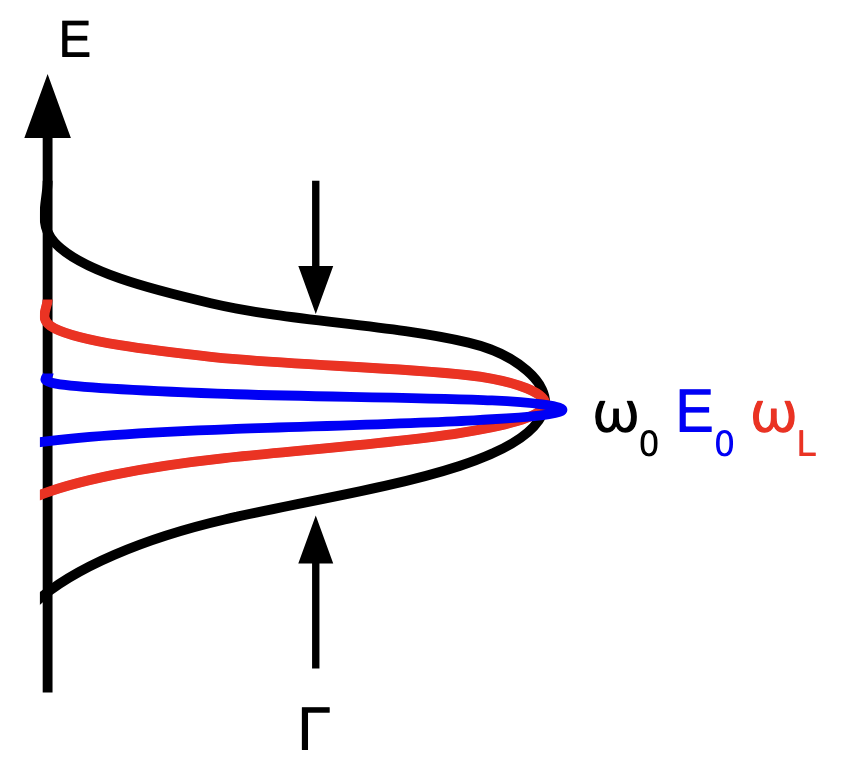
\includegraphics[scale = 0.7]{scheme_old.png}
\caption{Схема задачи с резонансным возбуждением~\cite{krainov2025}:
лазер, частота резонатора $\omega_0$ и трионный переход $E_0$ совпадают.
Накачка в $H$-поляризации, детектирование только в $V$-поляризации (кросс-поляризационная фильтрация).
$\Gamma$ --- скорость радиационного распада триона.}
\label{fig:scheme_old}
\end{figure}

В двухцветовой схеме~\cite{he2019} накачка ведётся двумя лазерными полями
на частотах $\omega_0 \pm \Omega_R$ --- боковые компоненты триплета Молоу,
где $\Omega_R$ --- частота осцилляций Раби.
Испускаемые КТ фотоны сосредоточены вблизи центральной компоненты $\omega_0$
и могут быть \emph{спектрально} отфильтрованы от накачки без поляризационного
ограничения.
Авторы экспериментально показали, что скорость счёта одиночных фотонов
при двухцветовой накачке в $\sim 2$ раза выше, чем при одноцветной,
при сохранении высокой чистоты однофотонного состояния.

Именно эта идея --- спектральное, а не поляризационное подавление лазерного излучения ---
лежит в основе нового подхода настоящей работы:
отстройка $\Delta = \omega_L - E_0 \neq 0$ позволяет детектировать
выходное поле во \emph{всех} поляризациях, что открывает доступ к
поляризационной запутанности.

\subsection{Точный расчёт: резонансное возбуждение двухуровневой системы $2\pi$-импульсом}

В работе~\cite{krainov2025} выполнен полный квантовый расчёт взаимодействия
двухуровневой системы (трион в КТ с резонатором) с резонансным когерентным
импульсом при площади импульса, кратной $2\pi$.

\medskip
\noindent\textbf{Схема задачи.}
Лазер настроен точно на трионный переход: $\omega_L = E_0 = \omega_0$.
Накачка --- в $H$-поляризации, детектирование --- в $V$-поляризации
(кросс-поляризационная фильтрация подавляет лазерный фон).
Гамильтониан взаимодействия:
\begin{equation}
    \hat{H} = E_0 \, \hat{a}^{\dag}_{+} \hat{a}_{+} + \omega_0 \, \hat{b}^{\dag}_{-} \hat{b}_{-}
    +  g \left( \hat{a}^{\dag}_{+} \hat{b}_{-} + \hat{a}_{+} \hat{b}^{\dag}_{-} \right),
\end{equation}
где $\hat{a}_{+}$ --- оператор трионного возбуждения,
$\hat{b}_{-}$ --- оператор фотона в $V$-поляризации,
$g$ --- константа связи с резонатором (Яблоновитт--Каммингс).

\medskip
\noindent\textbf{Метод и результат.}
Расчёт ведётся \emph{точно}: эволюция полного квантового состояния
поля (когерентный импульс в $H$-поляризации) и двухуровневой системы
вычисляется без каких-либо приближений на $g$.
Лишь на финальном этапе результат разворачивается до первого порядка по $g\tau$
для получения аналитических выражений.

Выходное состояние в $V$-поляризации принимает вид:
\begin{gather}
    \left| \psi_{out}^V \right\rangle \approx \cos \left( \frac{\theta}{2} \right) \left| 0 \right\rangle
    + \frac{i \delta - 1}{\sqrt{2}} \sin \left( \frac{\theta}{2} \right) \left| 1 \right\rangle
    + \frac{i \delta}{2} \cos \left( \frac{\theta}{2} \right) \left| 2 \right\rangle,
\end{gather}
где $\theta = g\tau\sqrt{N}$ --- площадь импульса ($N$ --- число фотонов в
когерентном состоянии), $\delta = g\tau \ll 1$ --- малый параметр,
определяющий вклад двухфотонного члена.
Нормированная корреляционная функция:
\begin{equation}
    g^{(2)}(0) = \frac{2\left|\delta\right|^2 \cos^2\!\left(\theta/2\right)}
    {\left(\sin^2\!\left(\theta/2\right) + \left|\delta\right|^2\right)^2}.
\end{equation}

При $\theta = 2\pi$ (полный оборот на сфере Блоха)
функция $g^{(2)}(0)$ может существенно превышать~1,
что означает суперпуассоновскую (суббунчинг) статистику фотонов ---
принципиально нелинейный эффект, недоступный для идеального однофотонного
источника, где $g^{(2)}(0) = 0$.

\medskip
\noindent\textbf{Ограничения предыдущего подхода.}
Поскольку детектирование ведётся только в $V$-поляризации,
выходное состояние~--- скалярное (одна поляризационная мода).
Поляризационная запутанность между фотонами не возникает и не
анализируется: ни concurrence, ни fidelity относительно Белловских
состояний не являются предметом исследования.
Именно это ограничение снимается в настоящей работе.

\newpage

\section{Теоретическая часть}

\subsection{Воспроизведение результатов~\cite{krainov2025} методом классического поля}

В работе~\cite{krainov2025} задача решается точно в рамках полной квантовой
теории: исходная матрица плотности системы включает квантовое поле обеих
поляризаций, а трактовка не вводит никаких приближений на $g$ вплоть до
финального разложения.

В настоящей работе используется альтернативный, но более экономичный подход:
поскольку число фотонов в $H$-поляризации велико ($N \gg 1$),
поле этой поляризации считается \emph{классическим}.
Тогда матрица плотности полной системы факторизуется:
\begin{gather}
    \hat{\rho}_{HV} = e^{\alpha \hat{b}^{\dag}_{H}}  \hat{\rho}_{V}  e^{\alpha^{*} \hat{b}_{H}},
\end{gather}
и после взятия $\mathrm{Tr}_H$ динамика сводится к уравнению
только на $V$-компоненту поля:
\begin{gather}
    i \frac{\partial \hat{\rho}_{V} }{\partial t} = \left[ \hat{H}_{V} ; \hat{\rho}_{V} \right].
\end{gather}
Эффективный гамильтониан, описывающий эволюцию в $V$-канале:
\begin{gather}
    \hat{H}_V = \Omega_R^{H} \left( \hat{d}^{\dag}_{\uparrow} \hat{a}_{\uparrow}
    + \hat{d}_{\uparrow} \hat{a}^{\dag}_{\uparrow} \right)
    + ig \left( \hat{b}_{V} \hat{d}^{\dag}_{\uparrow} \hat{a}_{\uparrow}
    - \hat{b}^{\dag}_{V} \hat{d}_{\uparrow} \hat{a}^{\dag}_{\uparrow} \right),
\end{gather}
где $\Omega_R^{H} \sim g\sqrt{N}$ --- частота осцилляций Раби от классического поля,
$g$ --- константа связи с резонатором.
Условие $N \gg 1$ даёт $\Omega_R^{H} \gg g$,
что позволяет ограничить фоковское пространство $V$-канала состояниями
с числом фотонов $n = 0$ и $n = 1$.

В отличие от предыдущей задачи, была рассмотрена более общая система с двумя
проекциями спина $\uparrow, \downarrow$.
В рамках данной системы базисные состояния:
\begin{gather}
    \hat{a}^{\dag}_{\uparrow} \left| 0 \right\rangle \, ; \, \hat{d}^{\dag}_{\uparrow} \left| 0 \right\rangle \, ; \, \hat{b}^{\dag}_{V} \hat{a}^{\dag}_{\uparrow} \left| 0 \right\rangle \, ; \, \hat{b}^{\dag}_{V} \hat{d}^{\dag}_{\uparrow} \left| 0 \right\rangle
\end{gather}
Базис соответствует спину $\uparrow$; аналогичный набор строится для $\downarrow$.
В этом базисе Гамильтониан записывается как:
\begin{gather}
    \hat{H} =
\begin{pmatrix}
    0 & \Omega_R & 0 & 0 \\
    \Omega_R & 0 & ig & 0 \\
    0 & -ig & 0 & \Omega_R \\
    0 & 0 & \Omega_R & 0
\end{pmatrix}
\end{gather}
И если выделить в нем блоки по фотонным состояниям:
\begin{gather}
    \hat{H} =
\begin{pmatrix}
    \hat{H_0} & \hat{V} \\
    \hat{V}^{\dag} & \hat{H_0}
\end{pmatrix}
\end{gather}
Теперь если переписать эту задачу в представлении взаимодействия, то получим:
\begin{gather}
    -i \frac{\partial}{\partial t } \left| \chi \right\rangle =
\begin{pmatrix}
    0 &  \hat{V_t} \\
     \hat{V_t}^{\dag} & 0
\end{pmatrix}
    \left| \chi \right\rangle \end{gather}
Где:
\begin{gather}
    \hat{V_t} = e^{i\hat{H_0}t} \hat{V} e^{-i\hat{H_0}t} \\ \nonumber
    \left| \psi \right\rangle =
\begin{pmatrix}
    e^{-i\hat{H_0}t} & 0 \\
    0 & e^{-i\hat{H_0}t}
\end{pmatrix}
    \left| \chi \right\rangle \\ \nonumber
    \left| \chi(0) \right\rangle = \left| \psi(0) \right\rangle = \hat{a}^{\dag}_{\uparrow} \left| 0 \right\rangle
\end{gather}
Решая эту задачу по теории возмущений в первом порядке по $g$, получаем ответ на $\left| \chi \right\rangle$:
\begin{gather}
    \left| \chi \right\rangle \approx \left( \hat{I} -i \int^t_0 d\tau
\begin{pmatrix}
    0 &  \hat{V_t} \\
     \hat{V_t}^{\dag} & 0
\end{pmatrix}
    \right) \left| \chi(0) \right\rangle
\end{gather}
Так как:
\begin{gather}
    -i \int^t_0 d\tau \hat{V_t}
\approx
\frac{gt}{2}
\begin{pmatrix}
    0 & 1 \\
    1 & 0
\end{pmatrix}
\end{gather}
То можно получить финальное выражение для $\left| \psi_{out} \right\rangle$:
\begin{gather}
    \left| \psi_{out} \right\rangle = \cos(\Omega_R t) \hat{a}^{\dag}_{\uparrow} \left| 0 \right\rangle  -i\sin(\Omega_R t) \hat{d}^{\dag}_{\uparrow} \left| 0 \right\rangle + gt \, i\sin(\Omega_R t) \hat{a}^{\dag}_{\uparrow} \hat{b}^{\dag}_{V} \left| 0 \right\rangle - \\ \nonumber
    - gt \, \cos(\Omega_R t) \hat{d}^{\dag}_{\uparrow} \hat{b}^{\dag}_{V} \left| 0 \right\rangle
\end{gather}
После того как трион высвечивается, а на детекторе мы регистрируем фотоны в $V$-поляризации:
\begin{gather}
    \left| \psi_{out} \right\rangle = \cos(\Omega_R t) \left| 0 \right\rangle  + \frac{i gt -1}{\sqrt{2}} \sin(\Omega_R t) \left| 1 \right\rangle + \frac{i gt}{2} \, \cos(\Omega_R t)  \left| 2 \right\rangle
\end{gather}

Этот результат полностью воспроизводит ответ, полученный точным квантовым
расчётом в~\cite{krainov2025}, что подтверждает корректность метода классического поля
в области $N \gg 1$.
Совпадение нетривиально: в точном подходе точка разложения по $g$ выбирается
в конце вычисления; метод классического поля даёт то же самое, вводя приближение
на более раннем этапе, но за счёт физически обоснованного условия $\Omega_R^H \gg g$.

Дальнейшие расчёты выполняются именно этим методом, поскольку он допускает
прямое обобщение на задачу с поперечным магнитным полем и нерезонансной накачкой.

\subsection{Новый подход: нерезонансная накачка и магнитное поле}
\par В рамках нового подхода система возбуждается \emph{нерезонансным} лазерным
импульсом с отстройкой $\Delta = \omega_L - E_0 \neq 0$.
Кроме того, к системе приложено поперечное (по отношению к оси роста КТ) магнитное поле
$\mathbf{B} = B_x \hat{x}$ (геометрия Фойгта).

Это принципиально меняет физику задачи по сравнению с~\cite{krainov2025}:
\begin{itemize}
    \item Отстройка $\Delta$ обеспечивает \emph{спектральное} отделение испущенных
    фотонов от лазерного фона, что позволяет \textbf{детектировать выходное поле
    во всех поляризациях} (а не только в $V$).
    \item Поперечное магнитное поле $B_x$ смешивает спиновые состояния
    $\left|\uparrow\right\rangle \leftrightarrow \left|\downarrow\right\rangle$ и
    $\left|\uparrow\uparrow\downarrow\right\rangle \leftrightarrow \left|\downarrow\downarrow\uparrow\right\rangle$,
    создавая связь между двумя кругово-поляризованными модами ($\sigma_+$ и $\sigma_-$).
    \item Совместное действие этих факторов приводит к тому, что двухфотонное
    выходное состояние оказывается \textbf{поляризационно-запутанным}:
    два испущенных фотона запутаны по своим поляризациям.
\end{itemize}

Схема установки показана на рис.~\ref{fig:scheme_new}.

\begin{figure}[h]
\centering
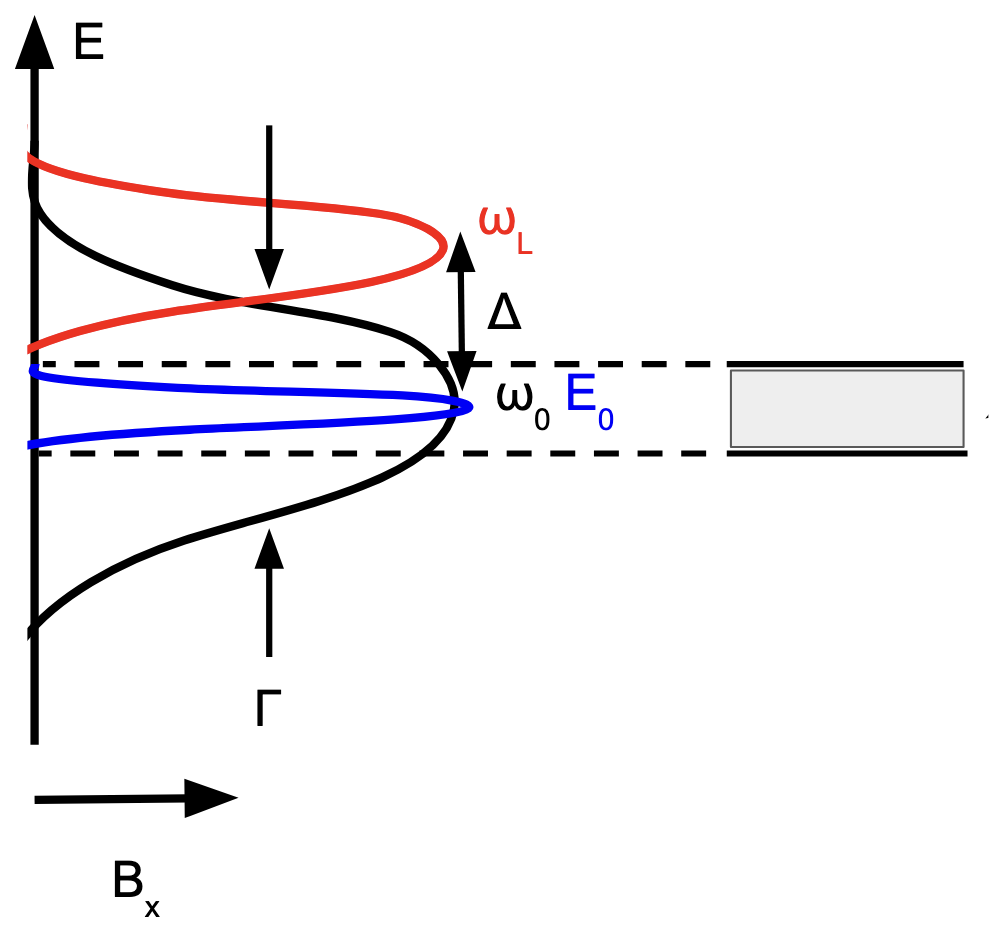
\includegraphics[scale = 0.7]{scheme_new.png}
\caption{Схема нового подхода: нерезонансная накачка с отстройкой $\Delta$ и поперечным
магнитным полем $B_x$.
$E_0$ --- энергия трионного перехода, $\omega_L$ --- частота лазера,
$\omega_0$ --- частота резонатора, $\Gamma$ --- скорость радиационного распада.
Прямоугольник справа --- область детектирования (все поляризации).}
\label{fig:scheme_new}
\end{figure}

\par
Такая система теперь описывается Гамильтонианом, учитывающим обе поляризации излучения, а также взаимодействие с магнитным полем:
\begin{gather}
    \hat{H}_{+} = \Delta \hat{d}^{\dag}_{\uparrow} \hat{d}_{\uparrow} + \Delta \hat{b}^{\dag}_{+} \hat{b}_{+} + \Omega_R \left( \hat{d}^{\dag}_{\uparrow} \hat{a}_{\uparrow}
    +  \hat{d}_{\uparrow} \hat{a}^{\dag}_{\uparrow} \right) + g \left( \hat{b}_{+} \hat{d}^{\dag}_{\uparrow} \hat{a}_{\uparrow}
    +  \hat{b}^{\dag}_{+} \hat{d}_{\uparrow} \hat{a}^{\dag}_{\uparrow} \right) \\ \nonumber
    \hat{H}_{-} = \Delta \hat{d}^{\dag}_{\downarrow} \hat{d}_{\downarrow} + \Delta \hat{b}^{\dag}_{-} \hat{b}_{-} + \Omega_R \left( \hat{d}^{\dag}_{\downarrow} \hat{a}_{\downarrow}
    +  \hat{d}_{\downarrow} \hat{a}^{\dag}_{\downarrow} \right) + g \left( \hat{b}_{-} \hat{d}^{\dag}_{\downarrow} \hat{a}_{\downarrow}
    +  \hat{b}^{\dag}_{-} \hat{d}_{\downarrow} \hat{a}^{\dag}_{\downarrow} \right) \\ \nonumber
    \hat{H}_{B} = \alpha B_x \left( \hat{a}^{\dag}_{\downarrow} \hat{a}_{\uparrow} + \hat{a}^{\dag}_{\uparrow} \hat{a}_{\downarrow}  \right) + \alpha B_z \left( \hat{a}^{\dag}_{\uparrow} \hat{a}_{\uparrow} - \hat{a}^{\dag}_{\downarrow} \hat{a}_{\downarrow}  \right) + \beta B_z \left( \hat{d}^{\dag}_{\uparrow} \hat{d}_{\uparrow} - \hat{d}^{\dag}_{\downarrow} \hat{d}_{\downarrow}  \right) \\ \nonumber
    \hat{H} = \hat{H}_{+} + \hat{H}_{-} + \hat{H}_{B} \nonumber
\end{gather}

Снова зафиксируем базис, ограничившись одним фотоном в Фоковском пространстве:
\begin{gather}
    \hat{a}^{\dag}_{\uparrow} \left| 0 \right\rangle \, ; \, \hat{a}^{\dag}_{\downarrow} \left| 0 \right\rangle \, ; \, \hat{d}^{\dag}_{\uparrow} \left| 0 \right\rangle \, ; \, \hat{d}^{\dag}_{\downarrow} \left| 0 \right\rangle \, ; \\ \nonumber
    \hat{b}^{\dag}_{+} \hat{a}^{\dag}_{\uparrow} \left| 0 \right\rangle \, ; \, \hat{b}^{\dag}_{-} \hat{a}^{\dag}_{\downarrow} \left| 0 \right\rangle \, ; \,
    \hat{b}^{\dag}_{+} \hat{d}^{\dag}_{\uparrow} \left| 0 \right\rangle \, ; \, \hat{b}^{\dag}_{-} \hat{d}^{\dag}_{\downarrow} \left| 0 \right\rangle \, ; \\ \nonumber
    \hat{b}^{\dag}_{-} \hat{a}^{\dag}_{\uparrow} \left| 0 \right\rangle \, ; \, \hat{b}^{\dag}_{+} \hat{a}^{\dag}_{\downarrow} \left| 0 \right\rangle \, ; \,
    \hat{b}^{\dag}_{-} \hat{d}^{\dag}_{\uparrow} \left| 0 \right\rangle \, ; \, \hat{b}^{\dag}_{+} \hat{d}^{\dag}_{\downarrow} \left| 0 \right\rangle
\end{gather}
В этом базисе наш Гамильтониан переписывается в блочном виде:
\begin{gather}
    \hat{H} =
\begin{pmatrix}
    \hat{H}_0 & \hat{g} & 0  \\
    \hat{g}^{\dag} & \hat{H}_0 + \hat{\Delta} & \alpha\hat{B}_x \\
    0 & \alpha \hat{B}_x^{\dag} & \hat{H}_0 + \hat{\Delta}
\end{pmatrix}
\end{gather}

Где:
\begin{gather}
    \hat{H}_{0} =
\begin{pmatrix}
    \alpha B_z & \alpha B_x & \Omega_R & 0 \\
    \alpha B_x & -\alpha B_z & 0 & \Omega_R \\
    \Omega_R & 0 & \beta B_z + \Delta & 0 \\
    0 & \Omega_R & 0 & -\beta B_z + \Delta
\end{pmatrix}
\\ \nonumber
    \hat{\Delta} =
\begin{pmatrix}
    \Delta & 0 & 0 & 0 \\
    0 & \Delta & 0 & 0 \\
    0 & 0 & \Delta & 0 \\
    0 & 0 & 0 & \Delta
\end{pmatrix}
\\ \nonumber
    \hat{g} =
\begin{pmatrix}
    0 & 0 & 0 & 0 \\
    0 & 0 & 0 & 0 \\
    g & 0 & 0 & 0 \\
    0 & g & 0 & 0
\end{pmatrix}
\\ \nonumber
    \alpha \hat{B}_x =
\begin{pmatrix}
    0 & \alpha B_x & 0 & 0 \\
    \alpha B_x & 0 & 0 & 0 \\
    0 & 0 & 0 & 0 \\
    0 & 0 & 0 & 0
\end{pmatrix}
\end{gather}

Решая задачу этим же методом по теории возмущений, но численно,
учитывая спиновую поляризацию триона по тепловому распределению:
\begin{gather}
    \hat{\rho}_{in} = f_{+x}\left( B/T \right) \left| x \right\rangle \left\langle x \right|  + f_{-x}\left( B/T \right)  \left| -x \right\rangle \left\langle -x \right|
\end{gather}
где
\begin{gather}
    f_{+x}\left( B/T \right) = \frac{e^{B/T}}{e^{B/T} + e^{-B/T}} \\ \nonumber
    f_{-x}\left( B/T \right) = \frac{e^{-B/T}}{e^{B/T} + e^{-B/T}}
\end{gather}
Уравнение эволюции на матрицу плотности учитывает фононы по механизму сбоя фазы:
\begin{gather}
    \frac{\partial \hat{\rho} }{\partial t} = -i \left[ \hat{H} ; \hat{\rho} \right] - \hat{L}(\hat{\rho}) \\ \nonumber
    \hat{L}(\hat{\rho}) = \gamma_{PD} \left( \hat{\rho} - \hat{\sigma}_z \hat{\rho} \hat{\sigma}_z \right) \\ \nonumber
    \hat{\rho}_{out} = \hat{S}_{\tau} \left( \hat{\rho}_{in} \right)
\end{gather}
Выделяя компоненты матрицы плотности, связанные с фотонными состояниями,
необходимо учитывать спиновую релаксацию электрона в магнитном поле.
\begin{gather}
    \hat{\rho}_{ph} = \hat{M}_{spin \,\, relax} \left(  \hat{\rho}_{out}  \right) = \\ \nonumber
    = f_{+x}\left( B/T \right) \left\langle x \right| \hat{\rho}_{out} \left| x \right\rangle + f_{-x}\left( B/T \right) \left\langle -x \right| \hat{\rho}_{out} \left| -x \right\rangle
\end{gather}
Матрица плотности содержит 3 типа фотонных состояний: с 0, 1 или 2 фотонами.
\begin{gather}
    \hat{\rho}_{ph} = \hat{\rho}_{0} + \hat{\rho}_{1} + \hat{\rho}_{2} \\ \nonumber
     p_1 = Tr\left( \hat{\rho}_{1} \right) \, \, \, ; \, \, \, p_2 = Tr\left( \hat{\rho}_{2} \right)
\end{gather}
Схематично 2-х фотонный сектор при $2\pi$-накачке выглядит следующим образом:

\begin{gather}
    \hat{\rho}^{(2\pi)}_2 \approx \left( g \tau \right)^2 \left( \frac{ \Omega_R^2}{ \Omega_R^2 + \Delta^2} \right)^2
\begin{pmatrix}
    1 & 0 & 0 & \tanh^2\left( B/T \right) \\
    0 & 0 & 0 & 0 \\
    0 & 0 & 0 & 0 \\
    \tanh^2\left( B/T \right) & 0 & 0 & 1
\end{pmatrix}
\end{gather}

Точный численный расчёт выполнен при следующих параметрах:
длительность импульса $\tau_p = 16$~пс,
$\Omega_R \tau_p = \pi$ (площадь $2\pi$-импульса), откуда $\Omega_R = 2\times10^{11}$~с$^{-1}$,
$\Omega_R \hbar \sim 10^2$~мкэВ,
$\Delta \sim \Gamma \sim 50$--$100$~мкэВ,
магнитное поле $B = 3$~Тл, $g_e = 0.5$, температура $T = 1$~К.

\begin{figure}[h]
\centering
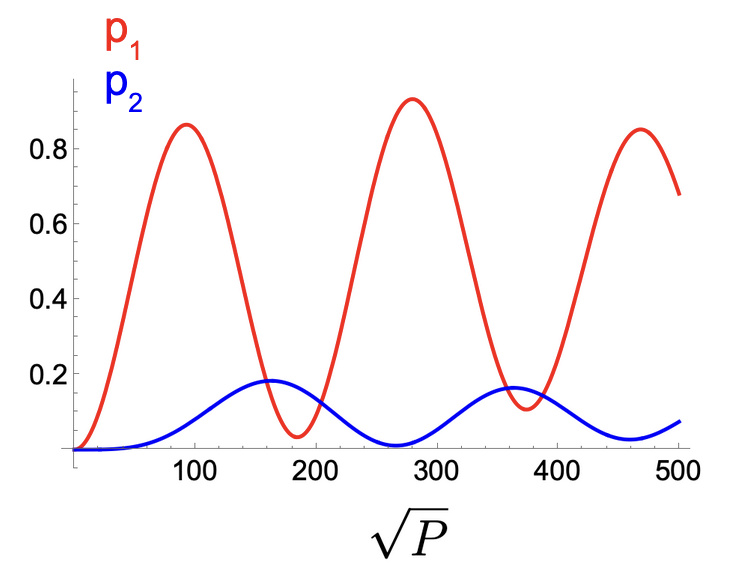
\includegraphics[scale = 0.7]{rabi.png}
\caption{Вероятности однофотонного ($p_1$, красная кривая) и двухфотонного ($p_2$, синяя кривая)
выходных состояний в зависимости от $\sqrt{P}$ --- квадратного корня из мощности накачки.
$p_1$ демонстрирует осцилляции Раби; вблизи $2\pi$-накачки ($\sqrt{P} \approx 260$)
наблюдается провал в $p_1$ и соответствующий пик в $p_2$,
что соответствует режиму двухфотонного испускания.
Параметры: $\tau_p = 16$~пс, $B = 3$~Тл, $T = 1$~К.}
\label{fig:rabi}
\end{figure}

\begin{figure}[h]
\centering
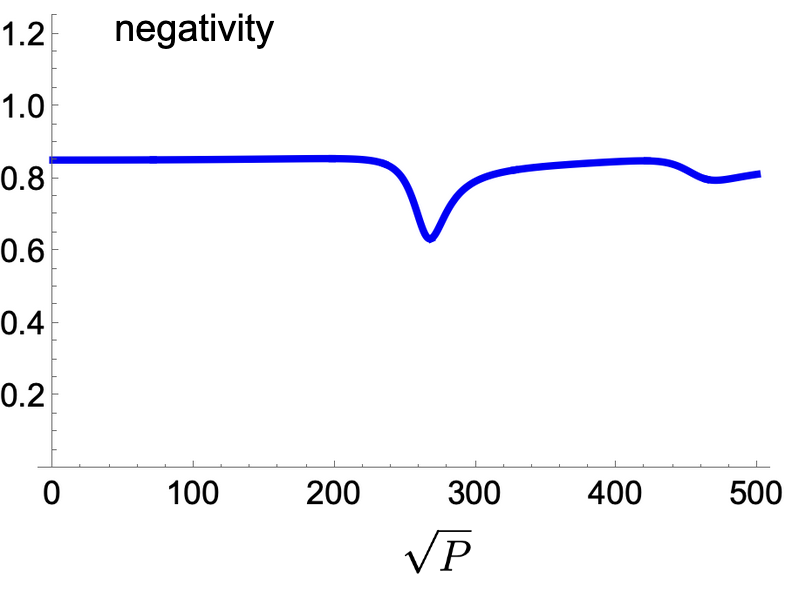
\includegraphics[scale = 0.7]{cuncurrence.png}
\caption{Concurrence двухфотонного выходного состояния как функция $\sqrt{P}$.
При малых и больших мощностях значение concurrence остаётся высоким
($C \approx 0.85$), что свидетельствует о высокой степени поляризационной запутанности.
Провал вблизи $\sqrt{P} \approx 270$ соответствует смене режима: при переходе
через $2\pi$-накачку структура двухфотонного состояния существенно меняется.
Параметры: $\tau_p = 16$~пс, $B = 3$~Тл, $T = 1$~К.}
\label{fig:concurrence}
\end{figure}

\begin{figure}[h]
\centering
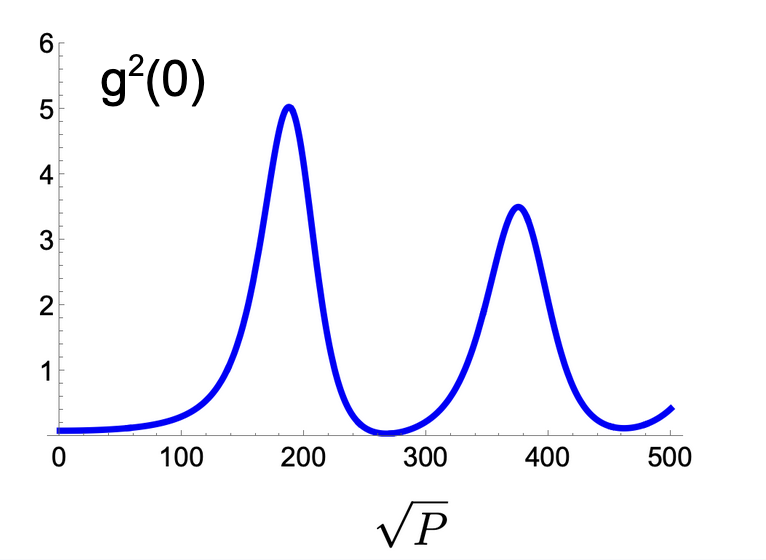
\includegraphics[scale = 0.7]{g20.png}
\caption{Нормированная корреляционная функция второго порядка $g^{(2)}(0)$
в зависимости от $\sqrt{P}$.
Пики вблизи $\sqrt{P} \approx 200$ и $380$ (значения $g^{(2)}(0) \approx 5$ и $3.5$)
указывают на суперпуассоновскую (суббунчинг) статистику фотонов,
характерную для режима многофотонного испускания.
В точках нечётных $\pi$-накачек $g^{(2)}(0) \to 0$ (источник близок к однофотонному).
Параметры: $\tau_p = 16$~пс, $B = 3$~Тл, $T = 1$~К.}
\label{fig:g20}
\end{figure}

\begin{figure}[h]
\centering
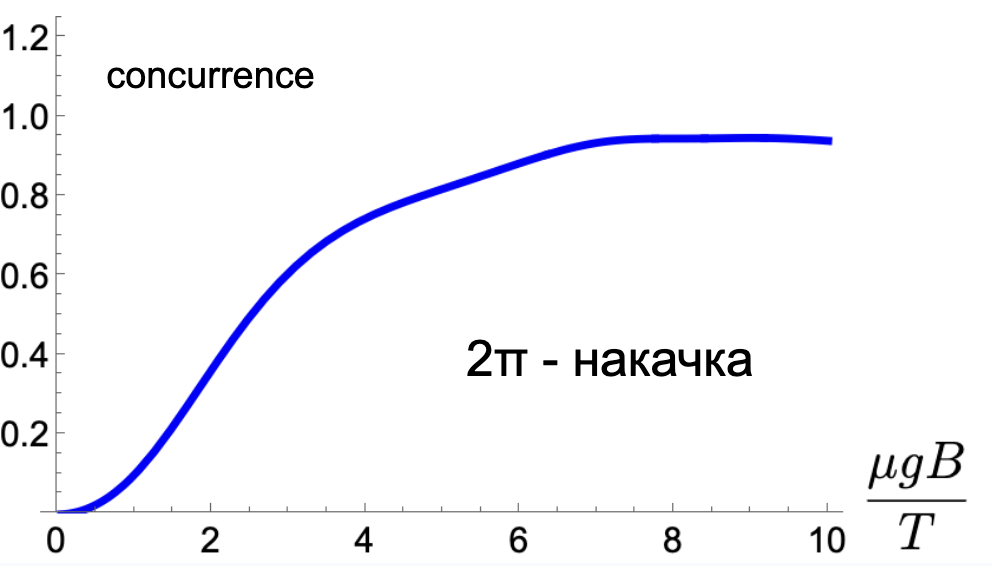
\includegraphics[scale = 0.7]{cuncurrence_ot_B.png}
\caption{Concurrence двухфотонного выходного состояния как функция безразмерного
параметра $\mu g_e B / T$ при $2\pi$-накачке.
С ростом магнитного поля запутанность монотонно возрастает от $0$ до $\approx 0.95$
и насыщается: при $\mu g_e B / T \gtrsim 7$ система практически полностью
поляризована, и состояние приближается к Белловскому.
Поведение обусловлено ростом $\tanh^2(B/T)$ в матрице плотности двухфотонного
сектора $\hat{\rho}_2^{(2\pi)}$.}
\label{fig:conc_B}
\end{figure}

\begin{figure}[h]
\centering
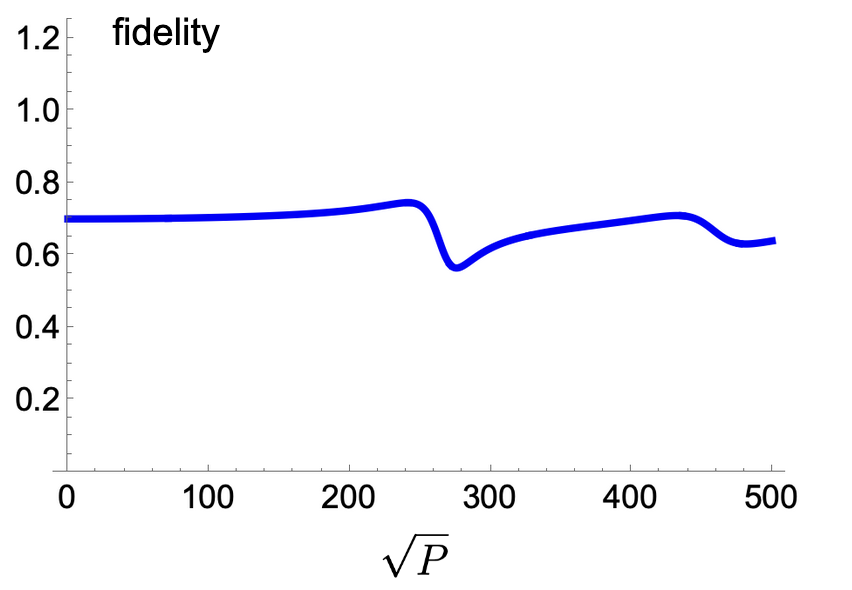
\includegraphics[scale = 0.7]{fidelity.png}
\caption{Верность (fidelity) $F$ двухфотонного выходного состояния
относительно Белловского состояния
$\left(\left|+_1 +_2\right\rangle + \left|-_1 -_2\right\rangle\right)/\sqrt{2}$
в зависимости от $\sqrt{P}$.
При малых мощностях $F \approx 0.70$, что заметно выше порога классической
сепарабельности ($F = 0.5$).
Провал вблизи $\sqrt{P} \approx 270$ коррелирует с провалом concurrence
и провалом в $p_1$ на рис.~\ref{fig:rabi}.
Параметры: $\tau_p = 16$~пс, $B = 3$~Тл, $T = 1$~К.}
\label{fig:fidelity}
\end{figure}


\section{Заключение}

В рамках данной работы исследована задача об управлении многофотонными
запутанными состояниями, испускаемыми двухуровневой системой (заряженная
квантовая точка с резидентным электроном в микрорезонаторе).

Работа является развитием результатов~\cite{krainov2025},
где задача о резонансном возбуждении системы $2\pi$-импульсом была решена
точно, а детектирование велось только в $V$-поляризации.
Предложенный в настоящей работе метод классического поля для $H$-поляризации
воспроизводит этот точный ответ в области $N \gg 1$,
что подтверждено прямым сравнением выходных состояний и функции $g^{(2)}(0)$.

Основным новым результатом является обобщение задачи на случай
нерезонансной накачки (отстройка $\Delta$) и поперечного магнитного поля
(геометрия Фойгта, $B_x$) с детектированием во \emph{всех} поляризациях.
Показано, что в этой конфигурации:
\begin{itemize}
    \item Двухфотонное выходное состояние является \textbf{поляризационно-запутанным}:
    concurrence достигает $C \approx 0.85$ при характерных параметрах
    $\tau_p = 16$~пс, $B = 3$~Тл, $T = 1$~К.
    \item Аналитически получено, что при $2\pi$-накачке двухфотонная матрица
    плотности пропорциональна $\tanh^2(B/T)$, монотонно стремясь к Белловскому
    состоянию с ростом $B/T$.
    \item Верность (fidelity) выходного состояния относительно симметричного
    Белловского состояния составляет $F \approx 0.70$ при малых мощностях
    и устойчива к изменению $\sqrt{P}$.
    \item Функция $g^{(2)}(0)$ демонстрирует пики суперпуассоновской статистики,
    коррелирующие с провалами в $p_1$ при площадях импульса, кратных $2\pi$.
\end{itemize}

Полученные результаты демонстрируют, что квантовая точка с резидентным
электроном при нерезонансном возбуждении и в поперечном магнитном поле
представляет собой управляемый источник поляризационно-запутанных фотонных
пар, перспективный для квантовых информационных технологий.

\section*{Список литературы}
\addcontentsline{toc}{section}{Список литературы}

\begin{thebibliography}{9}

\bibitem{krainov2025}
Krainov~I.\,V.
\textit{Coherent superposition of emitted and resonantly scattered photons from a two-level system driven by an even-$\pi$ pulse}.
Mesoscale and Nanoscale Physics, 2025.

\bibitem{scully1997}
Scully~M.\,O., Zubairy~M.\,S.
\textit{Quantum Optics}.
Cambridge University Press, 1997.

\bibitem{bonch1965}
Bonch-Bruevich~V.\,L.
\textit{Physics of Semiconductors}.
1965.

\bibitem{anselm1963}
Anselm~A.\,I.
\textit{Introduction to Semiconductor Theory}.
1963.

\bibitem{rakhlin2023}
Rakhlin~M.\,V., Galimov~A.\,I. et~al., Shubina~T.\,V., Toropov~A.\,A.
\textit{Journal of Luminescence},
\textbf{253}, 119496 (2023).

\bibitem{lindner2009}
Lindner~N.\,H., Rudolph~T.
\textit{Proposal for Pulsed On-Demand Sources of Photonic Cluster State Strings}.
Physical Review Letters, \textbf{103}, 113602 (2009).

\bibitem{he2019}
He~Y.-M., Wang~H. et~al.
\textit{Coherently driving a single quantum two-level system with dichromatic laser pulses}.
Nature Physics, \textbf{15}, 941--946 (2019).

\end{thebibliography}

\end{document}